% ══════════════════════════════════════════════════════════════════════════
% Why CFR converges — the complete proof, pedagogically
% Third volume of the PokerTrainer tutorial series.
% Build:  pdflatex cfr_convergence_proof.tex   (run twice for refs)
% ══════════════════════════════════════════════════════════════════════════
\documentclass[11pt,a4paper]{article}

\usepackage[utf8]{inputenc}
\usepackage[T1]{fontenc}
\usepackage{lmodern}
\usepackage[margin=2.2cm]{geometry}
\usepackage{amsmath,amssymb}
\usepackage[dvipsnames]{xcolor}
\usepackage{tikz}
\usetikzlibrary{arrows.meta,positioning,shapes.geometric,calc,fit,backgrounds}
\usepackage{listings}
\usepackage{tcolorbox}
\usepackage{booktabs}
\usepackage{enumitem}
\usepackage[colorlinks=true,linkcolor=MidnightBlue,urlcolor=MidnightBlue,citecolor=MidnightBlue]{hyperref}

\definecolor{accent}{RGB}{25,55,110}
\definecolor{heroG}{RGB}{20,110,60}
\definecolor{villR}{RGB}{160,40,40}
\definecolor{memO}{RGB}{190,110,10}
\definecolor{codebg}{RGB}{246,247,249}
\definecolor{codekw}{RGB}{0,80,160}
\definecolor{codecomment}{RGB}{100,120,100}
\definecolor{codestr}{RGB}{150,60,20}

\lstdefinestyle{py}{
  language=Python,
  basicstyle=\ttfamily\small,
  keywordstyle=\color{codekw}\bfseries,
  commentstyle=\color{codecomment}\itshape,
  stringstyle=\color{codestr},
  backgroundcolor=\color{codebg},
  frame=single, rulecolor=\color{black!25},
  framesep=6pt, xleftmargin=10pt, xrightmargin=4pt,
  showstringspaces=false,
  columns=fullflexible, keepspaces=true,
  breaklines=true
}

\newtcolorbox{intuition}{
  colback=blue!4, colframe=accent, boxrule=0.8pt, arc=2mm,
  title=\textbf{Intuition}, fonttitle=\color{white},
  left=6pt, right=6pt, top=4pt, bottom=4pt}
\newtcolorbox{defbox}{
  colback=black!3, colframe=black!50, boxrule=0.6pt, arc=2mm,
  left=6pt, right=6pt, top=4pt, bottom=4pt}
\newtcolorbox{thmbox}[1]{
  colback=heroG!5, colframe=heroG, boxrule=0.9pt, arc=2mm,
  title=\textbf{#1}, fonttitle=\color{white},
  left=6pt, right=6pt, top=4pt, bottom=4pt}
\newtcolorbox{trap}{
  colback=red!4, colframe=villR, boxrule=0.8pt, arc=2mm,
  title=\textbf{Watch out}, fonttitle=\color{white},
  left=6pt, right=6pt, top=4pt, bottom=4pt}

\newcommand{\E}{\mathbb{E}}
\newcommand{\pos}[1]{\left(#1\right)^{\!+}}

\setlength{\parskip}{4pt}
\setlength{\parindent}{0pt}

\title{\bfseries Why CFR converges\\[2mm]
\large The complete proof, built from scratch --- no prior knowledge assumed\\[1mm]
\normalsize Third volume of the PokerTrainer tutorial series}
\author{PokerTrainer documentation}
\date{June 2026}

\begin{document}
\maketitle

\begin{abstract}
The first volume of this series (\emph{Deep CFR, explained}) \emph{used} the
fact that CFR self-play converges to a Nash equilibrium. This volume
\emph{proves} it. The proof is genuinely beautiful and needs nothing beyond
careful algebra: three independent ingredients --- a $\sqrt{T}$ bound for
regret matching, a six-line ``folk theorem'' linking regret to equilibria, and
Zinkevich's decomposition of global regret into per-infoset regrets --- snap
together into the final theorem. Every step is motivated before it is taken,
every symbol is introduced before it is used, and a real numerical simulation
shows the theorem doing its work.
\end{abstract}

\tableofcontents
\newpage

% ════════════════════════════════════════════════════════════════════════════
\section{What we are going to prove, and the plan}
% ════════════════════════════════════════════════════════════════════════════

Here is the claim, first in plain words, then precisely.

\emph{In plain words:} two players repeatedly play a zero-sum game (such as
heads-up poker) against each other. At every decision point, each player runs
the same simple bookkeeping rule --- regret matching. Nobody is trying to
``converge'' to anything; each player just keeps updating its regrets. And
yet, the \textbf{average} of all the strategies each player has used becomes
arbitrarily close to a Nash equilibrium --- the unexploitable, ``GTO''
strategy --- with an error that shrinks like $1/\sqrt{T}$ after $T$
iterations.

\begin{thmbox}{Main theorem (Zinkevich et al.\ 2007, informal form)}
After $T$ iterations of CFR self-play in a two-player zero-sum game with
perfect recall, the pair of average strategies $(\bar\sigma_1,\bar\sigma_2)$
is an $\varepsilon$-Nash equilibrium with
\[
\varepsilon \;\le\; \frac{2\,\Delta\,|\mathcal{I}|\,\sqrt{A}}{\sqrt{T}},
\]
where $\Delta$ is the payoff range of the game, $|\mathcal{I}|$ the number of
information sets of one player, and $A$ the maximum number of actions at any
of them. In particular $\varepsilon \to 0$: average CFR self-play converges
to GTO.
\end{thmbox}

The proof has three independent ingredients, each interesting on its own:

\begin{center}
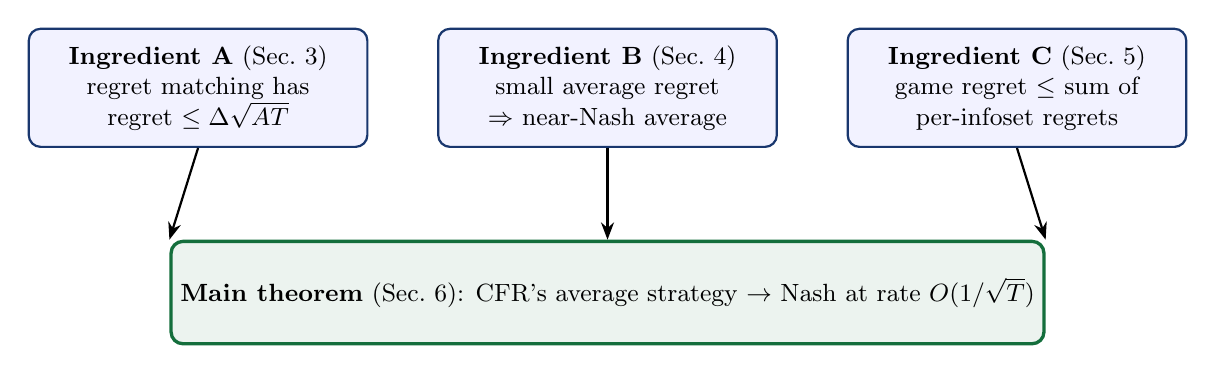
\begin{tikzpicture}[font=\small, >={Stealth[length=2.2mm]},
  ing/.style={rectangle, rounded corners=1.5mm, draw=accent, fill=blue!5, thick,
              align=center, minimum width=43mm, minimum height=15mm},
  main/.style={rectangle, rounded corners=1.5mm, draw=heroG, fill=heroG!8, very thick,
               align=center, minimum width=78mm, minimum height=13mm}]
  \node[ing] (A) at (0,0)
    {\textbf{Ingredient A} (Sec.~3)\\ regret matching has\\ regret $\le \Delta\sqrt{AT}$};
  \node[ing] (B) at (5.2,0)
    {\textbf{Ingredient B} (Sec.~4)\\ small average regret\\ $\Rightarrow$ near-Nash average};
  \node[ing] (C) at (10.4,0)
    {\textbf{Ingredient C} (Sec.~5)\\ game regret $\le$ sum of\\ per-infoset regrets};
  \node[main] (M) at (5.2,-2.6)
    {\textbf{Main theorem} (Sec.~6): CFR's average strategy $\to$ Nash at rate $O(1/\sqrt{T})$};
  \draw[->, thick] (A.south) -- (M.north west);
  \draw[->, thick] (B.south) -- (M.north);
  \draw[->, thick] (C.south) -- (M.north east);
\end{tikzpicture}
\end{center}

Notation we will use throughout (every symbol is re-introduced where it first
matters):

\begin{center}
\small
\begin{tabular}{@{}lll@{}}
\toprule
symbol & meaning & first used \\
\midrule
$a$, $A$           & an action; the number of available actions     & Sec.~2 \\
$t$, $T$           & current round; total number of rounds          & Sec.~2 \\
$u_t(a)$           & payoff action $a$ would have earned in round $t$ & Sec.~2 \\
$\sigma_t$         & our mixed strategy (probabilities) in round $t$ & Sec.~2 \\
$\Delta$           & payoff range: $\max u - \min u$                & Sec.~2 \\
$r_t(a)$, $R_T(a)$ & instantaneous / cumulative regret of $a$       & Sec.~2 \\
$x^{+}$            & positive part: $\max(x,0)$                     & Sec.~3 \\
$\bar\sigma$       & time-averaged strategy                         & Sec.~4 \\
$I$, $\mathcal{I}$ & an information set; the set of all of them     & Sec.~5 \\
$v(I,a)$           & counterfactual value of $a$ at $I$             & Sec.~5 \\
\bottomrule
\end{tabular}
\end{center}

% ════════════════════════════════════════════════════════════════════════════
\section{The arena: one repeated decision}
% ════════════════════════════════════════════════════════════════════════════

Forget game trees for now. The entire machinery is easiest to understand in
the simplest possible setting, and ingredient A lives there entirely.

You face the \emph{same} decision over and over: rounds $t = 1, 2, \dots, T$.
In each round you must choose among $A$ actions, and you are allowed to
randomize: you pick a probability vector $\sigma_t$ (your \emph{mixed
strategy}) and play a draw from it. \textbf{After} the round, the environment
reveals what every action would have paid this round: a vector $u_t$, with
$u_t(a)$ the payoff of action $a$. Crucially, we make \emph{no assumption} on
how $u_t$ is produced --- it may depend on your past play, it may be chosen by
an adversary who knows your algorithm. The only structure is a bounded range:
all payoffs live in an interval of width $\Delta$.

Your \emph{expected} payoff in round $t$ is
$\langle\sigma_t, u_t\rangle = \sum_a \sigma_t(a)\,u_t(a)$.

\begin{defbox}
\textbf{Regret.} The \emph{instantaneous regret} of action $a$ in round $t$
is how much better $a$ would have done than what you actually did:
\[
r_t(a) \;=\; u_t(a) - \langle\sigma_t, u_t\rangle .
\]
The \emph{cumulative regret} after $T$ rounds is
$R_T(a) = \sum_{t=1}^{T} r_t(a)$, and your \emph{(external) regret} is
$R_T = \max_a R_T(a)$: how much you lost compared to the best
\emph{single fixed action} chosen with hindsight.
\end{defbox}

Note two easy facts we will use constantly. First, since both $u_t(a)$ and
$\langle\sigma_t,u_t\rangle$ lie in the same interval of width $\Delta$,
every instantaneous regret is bounded: $|r_t(a)| \le \Delta$. Second, the
strategy-weighted average of the instantaneous regrets is \emph{always zero}:
\[
\sum_a \sigma_t(a)\, r_t(a)
 = \sum_a \sigma_t(a)\,u_t(a) - \langle\sigma_t,u_t\rangle \cdot \underbrace{\textstyle\sum_a \sigma_t(a)}_{=1} = 0 .
\]
Regret is a \emph{relative} quantity --- you cannot regret everything at once.

\begin{intuition}
Why is ``low regret against the best fixed action'' the right goal, rather
than ``high payoff''? Because against an unknown, possibly adversarial
environment, payoff itself is not controllable --- the environment can always
pay you nothing. What \emph{is} controllable is the gap to the best hindsight
action. And as Section~4 shows, in a two-player zero-sum game this modest
goal is secretly equivalent to finding an equilibrium.
\end{intuition}

\textbf{Regret matching} (Hart \& Mas-Colell 2000) is the bookkeeping rule
from volume one: play each action proportionally to its positive cumulative
regret, $\sigma_{t+1}(a) = R_t^{+}(a) \big/ \sum_b R_t^{+}(b)$, and play
anything (say uniform) if no regret is positive. Our question for the next
section: \emph{how big can $R_T$ get under regret matching?}

% ════════════════════════════════════════════════════════════════════════════
\section{Ingredient A: regret matching's regret grows only like $\sqrt{T}$}
% ════════════════════════════════════════════════════════════════════════════

\begin{thmbox}{Theorem A (Hart \& Mas-Colell 2000)}
Against \emph{any} sequence of payoff vectors with range $\Delta$, regret
matching guarantees
\[
R_T \;=\; \max_a R_T(a) \;\le\; \Delta\,\sqrt{A\,T}.
\]
Hence the \emph{average} regret $R_T/T \le \Delta\sqrt{A/T}$ vanishes as
$T \to \infty$.
\end{thmbox}

A bound that holds against any adversary, for such a naive rule, should feel
surprising. The proof is three small steps. The object to watch is the
\textbf{potential}
\[
\Phi_T \;=\; \sum_a \bigl(R_T^{+}(a)\bigr)^2,
\]
the squared length of the \emph{clipped} regret vector. We will show
$\Phi$ can only grow by a bounded amount per round --- which forces every
individual regret to stay $O(\sqrt{T})$.

\subsection{Step 1: the key cancellation}

\begin{thmbox}{Lemma 1 (the regret-matching identity)}
If $\sigma_{t+1}$ is chosen by regret matching from $R_t$, then
\[
\sum_a R_t^{+}(a)\; r_{t+1}(a) \;=\; 0 .
\]
\end{thmbox}

\emph{Proof.} If all regrets are $\le 0$ the left side is trivially zero
(every $R^{+}_t(a)=0$). Otherwise let $Z = \sum_b R_t^{+}(b) > 0$, so
$\sigma_{t+1}(a) = R_t^{+}(a)/Z$. Then
\[
\sum_a R_t^{+}(a)\,r_{t+1}(a)
= \sum_a R_t^{+}(a)\,u_{t+1}(a)
\;-\; \Bigl(\sum_a R_t^{+}(a)\Bigr)\,\langle\sigma_{t+1},u_{t+1}\rangle .
\]
The second term is
$Z \cdot \sum_a \frac{R_t^{+}(a)}{Z} u_{t+1}(a) = \sum_a R_t^{+}(a)u_{t+1}(a)$
--- identical to the first. They cancel. $\square$

\begin{center}
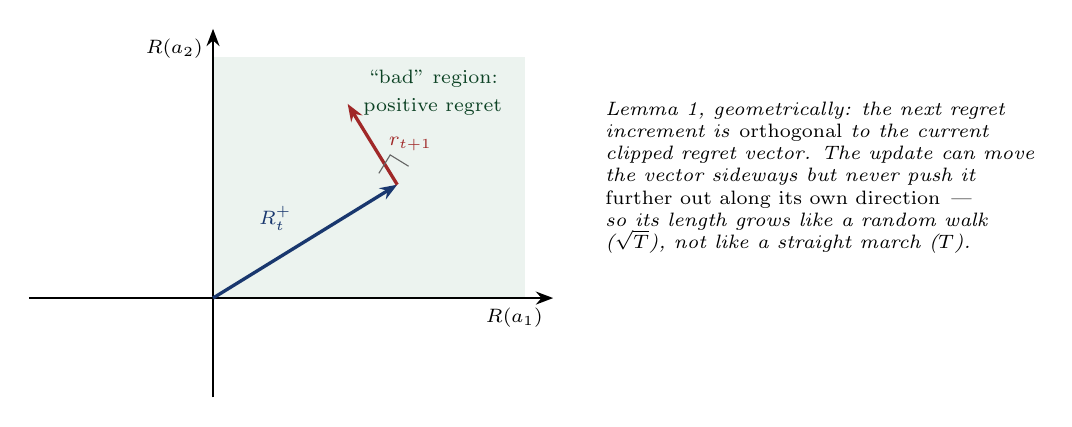
\begin{tikzpicture}[font=\small, >={Stealth[length=2.2mm]}, scale=0.9]
  % positive orthant
  \fill[heroG!8] (0,0) rectangle (4.4,3.4);
  \draw[->, thick] (-2.6,0) -- (4.8,0) node[below left, font=\scriptsize]{$R(a_1)$};
  \draw[->, thick] (0,-1.4) -- (0,3.8) node[below left, font=\scriptsize]{$R(a_2)$};
  \node[font=\scriptsize, color=heroG!60!black] at (3.1,3.1) {``bad'' region:};
  \node[font=\scriptsize, color=heroG!60!black] at (3.1,2.7) {positive regret};
  % current regret vector
  \draw[->, very thick, accent] (0,0) -- (2.6,1.6)
      node[midway, above left=0pt and 1pt, font=\scriptsize]{$R_t^{+}$};
  % increment, orthogonal
  \draw[->, very thick, villR] (2.6,1.6) -- (1.9,2.74)
      node[midway, right=2pt, font=\scriptsize]{$r_{t+1}$};
  \draw[black!60] (2.34,1.76) -- (2.5,2.02) -- (2.76,1.86); % right-angle mark
  \node[font=\scriptsize\itshape, align=left, anchor=west] at (5.4,1.7)
    {Lemma 1, geometrically: the next regret\\
     increment is \emph{orthogonal} to the current\\
     clipped regret vector. The update can move\\
     the vector sideways but never push it\\
     \emph{further out along its own direction} ---\\
     so its length grows like a random walk\\
     ($\sqrt{T}$), not like a straight march ($T$).};
\end{tikzpicture}
\end{center}

\subsection{Step 2: clipping never hurts}

\begin{thmbox}{Lemma 2 (clipping inequality)}
For any real numbers $x, y$:\quad
$\bigl(\pos{x+y}\bigr)^2 \;\le\; \bigl(x^{+} + y\bigr)^2$.
\end{thmbox}

\emph{Proof.} If $x + y \le 0$ the left side is $0$ and the right side is a
square, hence $\ge 0$. If $x+y > 0$, then since $x^{+} \ge x$ we have
$x^{+}+y \ge x+y > 0$, and squaring preserves order on positives. $\square$

\subsection{Step 3: the potential argument}

Now bound the growth of $\Phi$. For each action $a$, apply Lemma 2 with
$x = R_t(a)$, $y = r_{t+1}(a)$, and sum over $a$:
\[
\Phi_{t+1}
= \sum_a \bigl(\pos{R_t(a) + r_{t+1}(a)}\bigr)^2
\;\le\; \sum_a \bigl(R_t^{+}(a) + r_{t+1}(a)\bigr)^2
= \Phi_t
\;+\; 2\underbrace{\sum_a R_t^{+}(a)\,r_{t+1}(a)}_{=\,0 \text{ (Lemma 1)}}
\;+\; \sum_a r_{t+1}(a)^2 .
\]
The middle term --- the only one that could grow linearly --- is annihilated
by Lemma 1. The last term is at most $A\Delta^2$ because each
$|r_{t+1}(a)| \le \Delta$. So
\[
\Phi_{t+1} \le \Phi_t + A\Delta^2
\qquad\Longrightarrow\qquad
\Phi_T \le T\,A\,\Delta^2 .
\]
Finally, a single squared coordinate is at most the whole sum of squares:
\[
R_T(a) \;\le\; R_T^{+}(a) \;\le\; \sqrt{\Phi_T} \;\le\; \Delta\sqrt{A\,T}
\qquad\text{for every } a . \qquad\blacksquare
\]

\begin{intuition}
The whole theorem is the picture under Lemma 1. The clipped regret vector
performs a dance in which every step is \emph{perpendicular} to its current
position (plus a bounded-length correction from clipping). Perpendicular
steps of bounded size grow a vector's \emph{squared} length by a constant per
step --- the same reason a random walk wanders only $\sqrt{T}$ from home.
``$\sqrt{T}$ regret'' is not a coincidence of regret matching; it is the
signature of any algorithm that manages to keep its updates orthogonal to
its accumulated mistakes.
\end{intuition}

\subsection{Watching the theorem work}

The table below is a \emph{real} simulation (seed 7) of two regret matchers
playing rock--paper--scissors against each other with sampled actions
($\Delta = 2$, $A = 3$, so Theorem A promises $R_T \le 2\sqrt{3T}$):

\begin{center}
\small
\begin{tabular}{@{}rrrrr@{}}
\toprule
$T$ & $\max_a R_T(a)$ & bound $2\sqrt{3T}$ & $R_T/T$ & avg.\ strategy (R,\,P,\,S) \\
\midrule
10      & 3.3   & 11.0   & 0.327  & (0.103,\;0.730,\;0.167) \\
100     & 9.9   & 34.6   & 0.099  & (0.346,\;0.399,\;0.255) \\
1\,000  & 28.3  & 109.5  & 0.028  & (0.355,\;0.316,\;0.329) \\
10\,000 & 92.0  & 346.4  & 0.009  & (0.347,\;0.330,\;0.323) \\
100\,000& 351.8 & 1095.4 & 0.004  & (0.336,\;0.328,\;0.336) \\
\bottomrule
\end{tabular}
\end{center}

Three things to see. (1) Regret grows, but each $\times 10$ in $T$ multiplies
it by only ${\approx}3.2 \approx \sqrt{10}$ --- the square-root law, well
inside the bound. (2) \emph{Average} regret melts away. (3) The average
strategy approaches $(\tfrac13,\tfrac13,\tfrac13)$, the Nash equilibrium of
RPS --- even though at $T{=}10$ the player was a wild Paper-spammer. That
last observation is not explained by Theorem A at all. It is the subject of
ingredient B.

% ════════════════════════════════════════════════════════════════════════════
\section{Ingredient B: low regret $\Rightarrow$ near-equilibrium (the folk
theorem)}
% ════════════════════════════════════════════════════════════════════════════

Now let the ``environment'' be another player. Two players repeatedly play a
\textbf{zero-sum} game: player 1 picks mixed strategy $\sigma_1^t$, player 2
picks $\sigma_2^t$, and player 1's expected payoff is the bilinear
$u(\sigma_1^t, \sigma_2^t)$, with player 2 receiving its negation. Each
player measures its own regret exactly as in Section~2 (for player 1 in round
$t$, the payoff vector is $u_t(a) = u(a, \sigma_2^t)$ --- what each of my
actions would have earned against what the opponent actually played).

\begin{defbox}
\textbf{$\varepsilon$-Nash equilibrium.} A profile
$(\bar\sigma_1,\bar\sigma_2)$ such that neither player can gain more than
$\varepsilon$ by deviating unilaterally:
$u(\sigma_1',\bar\sigma_2) \le u(\bar\sigma_1,\bar\sigma_2) + \varepsilon$
for every $\sigma_1'$, and symmetrically for player 2. The smallest such
$\varepsilon$ is the profile's \emph{exploitability}: how much a perfect
counter-strategy could win above the equilibrium value.
\end{defbox}

\begin{defbox}
\textbf{Average strategy.} $\bar\sigma_i = \frac1T\sum_{t=1}^{T}\sigma_i^t$ ---
the mixture that plays a uniformly random past round's strategy. The single
property we need is linearity of expected payoff in each argument:
\[
\frac1T \sum_{t=1}^{T} u(\sigma_1', \sigma_2^t) \;=\;
u\Bigl(\sigma_1', \tfrac1T\textstyle\sum_t \sigma_2^t\Bigr) \;=\;
u(\sigma_1', \bar\sigma_2).
\]
\emph{Playing against the average of my opponent's past selves is the same as
playing against each past self with probability $1/T$.}
\end{defbox}

\begin{thmbox}{Theorem B (the folk theorem of online learning)}
If after $T$ rounds player 1's average regret is at most $\varepsilon_1$ and
player 2's is at most $\varepsilon_2$, then $(\bar\sigma_1, \bar\sigma_2)$ is
an $(\varepsilon_1{+}\varepsilon_2)$-Nash equilibrium.
\end{thmbox}

\emph{Proof.} Let $\bar v = \frac1T\sum_t u(\sigma_1^t,\sigma_2^t)$ be the
average realized payoff (to player 1). Player 1's regret guarantee says: for
\emph{every} alternative $\sigma_1'$,
\[
\frac1T\sum_t u(\sigma_1', \sigma_2^t) - \bar v \;\le\; \varepsilon_1
\qquad\overset{\text{linearity}}{\Longrightarrow}\qquad
u(\sigma_1', \bar\sigma_2) \;\le\; \bar v + \varepsilon_1 .
\tag{$*$}
\]
Player 2's guarantee, written in player-1 payoffs (player 2 \emph{earns}
$-u$, so low regret for 2 means no $\sigma_2'$ pushes $u$ much \emph{below}
$\bar v$):
\[
u(\bar\sigma_1, \sigma_2') \;\ge\; \bar v - \varepsilon_2
\qquad\text{for every } \sigma_2' .
\tag{$**$}
\]
Now read the two lines together. Setting $\sigma_2' = \bar\sigma_2$ in
$(**)$: $u(\bar\sigma_1,\bar\sigma_2) \ge \bar v - \varepsilon_2$. Hence for
every deviation $\sigma_1'$:
\[
u(\sigma_1', \bar\sigma_2)
\;\overset{(*)}{\le}\; \bar v + \varepsilon_1
\;\le\; u(\bar\sigma_1, \bar\sigma_2) + \varepsilon_1 + \varepsilon_2 .
\]
Player 1 cannot gain more than $\varepsilon_1{+}\varepsilon_2$ by deviating;
the argument for player 2 is the mirror image. $\square$

\begin{intuition}
Six lines, and they explain the third column of our RPS table. Each player's
regret guarantee constrains the \emph{opponent's average}: ``my regret is
small'' literally means ``no fixed strategy beats the average of what my
opponent has been doing by much''. Two such statements, one per player, pin
the average profile to the equilibrium from both sides. Note also \emph{what
failed}: nothing forces $\sigma^T$ itself --- the current strategy --- to be
anywhere near Nash. It is the \emph{averages} that are squeezed. This is the
deep reason Deep CFR must train a separate average-policy network, and why
judging a mid-training CFR run by its current strategy is a mistake.
\end{intuition}

\begin{trap}
In an \emph{extensive-form} game (a game tree), ``the average strategy''
must be defined so that the linearity step in the proof still holds. The
correct object weights each round's behavior at an infoset by that round's
probability of \emph{reaching} the infoset under the player's own strategy
--- averaging the action probabilities naively would break $(*)$. This is
exactly why the CFR pseudo-code in the companion volumes accumulates
\texttt{S[I] += reach[p] * sigma}: that reach factor is not an implementation
detail, it is the hypothesis of Theorem B.
\end{trap}

% ════════════════════════════════════════════════════════════════════════════
\section{Ingredient C: from one decision to a whole game tree}
% ════════════════════════════════════════════════════════════════════════════

Ingredients A and B already prove convergence for games with \emph{one}
simultaneous decision (like RPS). Poker, however, is a \emph{tree} of
decisions with hidden information. The bridge is the conceptual heart of the
CFR paper: define a \emph{local} regret at every infoset such that
\textbf{(i)} each local regret can be driven down by an independent regret
matcher (ingredient A applies), and \textbf{(ii)} the local regrets jointly
control the only thing we actually care about --- the global, whole-game
regret that ingredient B consumes.

\begin{defbox}
\textbf{Counterfactual value and counterfactual regret.} Fix the current
strategy profile $\sigma^t$ and an infoset $I$ belonging to player $i$. The
\emph{counterfactual value} $v(I, a)$ is the expected payoff to $i$ for
playing $a$ at $I$, where the probability of being at $I$ is weighted only by
the \emph{others'} contribution (opponent and chance) --- as if player $i$
had steered toward $I$ on purpose. The \emph{immediate counterfactual
regret} at $I$ after $T$ rounds is then exactly a Section-2 regret built from
these values:
\[
R_T^{\mathrm{imm}}(I) \;=\; \max_a \sum_{t=1}^{T}
\Bigl( v^t(I,a) - \textstyle\sum_b \sigma^t(I,b)\, v^t(I,b) \Bigr).
\]
CFR is, by definition, the algorithm that runs one regret matcher per infoset
on these quantities.
\end{defbox}

Because the counterfactual reach weight of the others is at most $1$, each
$v(I,a)$ has range at most $\Delta$, so Theorem A applies verbatim at each
infoset:
\[
R_T^{\mathrm{imm}}(I) \;\le\; \Delta\sqrt{A\,T}
\qquad \text{for every } I . \tag{A applied locally}
\]

What remains is the decomposition: local control implies global control.

\begin{thmbox}{Theorem C (Zinkevich et al.\ 2007, regret decomposition)}
For a player with perfect recall, the whole-game external regret is bounded
by the sum of clipped immediate counterfactual regrets:
\[
R_T^{\mathrm{game}} \;\le\; \sum_{I \in \mathcal{I}}
\pos{R_T^{\mathrm{imm}}(I)} .
\]
\end{thmbox}

\emph{Proof idea, made precise by induction.} The global regret compares
your play to the best \emph{deviation strategy} $\sigma'$ --- a full
alternative plan that may change the action at \emph{every} infoset at once.
The key observation is that any such plan can be charged, infoset by infoset,
to local regrets.

Define, for each infoset $I$ of the player, the \emph{at-and-below regret}
$R_T^{\mathrm{full}}(I)$: the best gain achievable by deviating at $I$
\emph{and at any of the player's infosets below it}, weighted
counterfactually as above. With perfect recall, the player's infosets form a
tree (each infoset remembers its own past, so it has a unique parent), and we
can induct from the leaves upward:

\begin{center}
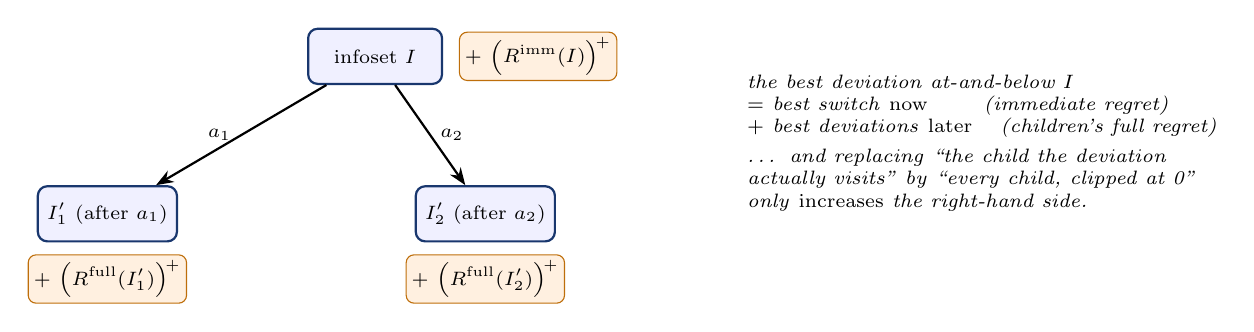
\begin{tikzpicture}[font=\small, >={Stealth[length=2.2mm]},
  iset/.style={rectangle, rounded corners=1.2mm, draw=accent, fill=blue!6, thick,
               minimum width=17mm, minimum height=7mm, font=\scriptsize, align=center},
  chip/.style={rectangle, rounded corners=1mm, draw=memO, fill=orange!12,
               font=\scriptsize, inner sep=2pt}]
  \node[iset] (root) at (0,3.0) {infoset $I$};
  \node[chip, right=2mm of root] {$+\,\pos{R^{\mathrm{imm}}(I)}$};
  \node[iset] (c1) at (-3.4,1.0) {$I_1'$ (after $a_1$)};
  \node[iset] (c2) at (1.4,1.0) {$I_2'$ (after $a_2$)};
  \node[chip, below=1.5mm of c1] {$+\,\pos{R^{\mathrm{full}}(I_1')}$};
  \node[chip, below=1.5mm of c2] {$+\,\pos{R^{\mathrm{full}}(I_2')}$};
  \draw[->, thick] (root) -- node[left, font=\scriptsize]{$a_1$} (c1);
  \draw[->, thick] (root) -- node[right, font=\scriptsize]{$a_2$} (c2);
  \node[font=\scriptsize\itshape, align=left, anchor=west] at (4.6,1.9)
    {the best deviation at-and-below $I$\\
     $=$ best switch \emph{now}\hspace{2.4em}(immediate regret)\\
     $+$ best deviations \emph{later}\hspace{1.2em}(children's full regret)\\[1mm]
     \dots{} and replacing ``the child the deviation\\
     actually visits'' by ``every child, clipped at 0''\\
     only \emph{increases} the right-hand side.};
\end{tikzpicture}
\end{center}

Formally, one shows for every infoset $I$:
\[
R_T^{\mathrm{full}}(I) \;\le\; R_T^{\mathrm{imm}}(I)
\;+\; \sum_{I' \in \mathrm{succ}(I)} \pos{R_T^{\mathrm{full}}(I')},
\]
where $\mathrm{succ}(I)$ are the player's next infosets reachable from $I$.
The reasoning: a deviation plan at $I$ first gains whatever its action switch
at $I$ alone gains (at most $R_T^{\mathrm{imm}}(I)$, by definition of the
immediate regret), and then gains whatever its sub-plan gains below ---
but each below-gain is counted in that child's own full regret, and clipping
at zero lets us include \emph{all} children instead of only the ones the plan
steers toward (adding non-negative terms can only help the bound). Taking
positive parts of both sides preserves the inequality, and unrolling the
recursion from the leaves (where
$R^{\mathrm{full}} = R^{\mathrm{imm}}$) up to the root turns the nested sums
into one flat sum over all infosets. At the root, the at-and-below regret
\emph{is} the whole-game regret. $\square$

\begin{intuition}
Why must the local values be \emph{counterfactual} --- weighted by the
others' reach only? Look at where the induction charges a deviation's gain:
to the local regret \emph{at the infoset where the deviation acts}. For that
charge to be honest, the local regret must already account for ``how often
does play arrive here if \emph{I} try to come here'' --- i.e.\ it must not be
discounted by the player's own (possibly deviating) probabilities, which the
plan is free to change. Weighting by the others' reach makes the local
ledger deviation-proof, and it is precisely the
\texttt{reach[1-p]} factor in the pseudo-code of the companion volumes.
Perfect recall is what makes the infosets a \emph{tree} so the induction is
well-founded --- without it, deviations could ``merge'' paths and gains would
be double-counted.
\end{intuition}

% ════════════════════════════════════════════════════════════════════════════
\section{The assembly: proving the main theorem}
% ════════════════════════════════════════════════════════════════════════════

Everything is on the table; the final proof is a four-line chain. Consider
player $i$ after $T$ iterations of CFR self-play:

\[
\frac{R_T^{\mathrm{game}}}{T}
\;\overset{\text{(C)}}{\le}\;
\frac{1}{T}\sum_{I\in\mathcal{I}} \pos{R_T^{\mathrm{imm}}(I)}
\;\overset{\text{(A)}}{\le}\;
\frac{|\mathcal{I}|\,\Delta\sqrt{A\,T}}{T}
\;=\;
\frac{|\mathcal{I}|\,\Delta\sqrt{A}}{\sqrt{T}}
\;=:\; \varepsilon_i .
\]

Both players run the same procedure, so both average regrets are at most
this $\varepsilon_i$. Feed them to Theorem B:

\begin{thmbox}{Main theorem, assembled}
After $T$ CFR iterations, $(\bar\sigma_1, \bar\sigma_2)$ is an
$\varepsilon$-Nash equilibrium with
\[
\varepsilon \;\le\; \varepsilon_1 + \varepsilon_2
\;\le\; \frac{2\,\Delta\,|\mathcal{I}|\,\sqrt{A}}{\sqrt{T}}
\;\xrightarrow[T\to\infty]{}\; 0 . \qquad\blacksquare
\]
\end{thmbox}

Each inequality is one ingredient, and each ingredient carries one idea:

\begin{center}
\small
\begin{tabular}{@{}lll@{}}
\toprule
step & ingredient & the one idea \\
\midrule
game regret $\le$ sum of local regrets & C (decomposition) & charge deviations infoset-by-infoset \\
each local regret $\le \Delta\sqrt{AT}$ & A (regret matching) & updates orthogonal to mistakes \\
small avg.\ regret $\Rightarrow$ near-Nash & B (folk theorem) & two regret bounds pin the average \\
\bottomrule
\end{tabular}
\end{center}

% ════════════════════════════════════════════════════════════════════════════
\section{What the proof promises --- and what it does not}
% ════════════════════════════════════════════════════════════════════════════

Reading the fine print of a theorem is half the value of proving it.

\textbf{It is the average, never the current strategy.} Nothing anywhere
constrains $\sigma^T$; the RPS table showed a Paper-spamming current strategy
coexisting with a converging average. Practical corollaries: Deep CFR's
deliverable is the policy network trained on the strategy memory, and
mid-training sanity checks must target average behavior (or known
equilibria, like this project's stage-1 push/fold oracle).

\textbf{The bound is worst-case and dimension-aware.} $\varepsilon$ scales
with $|\mathcal{I}|$ (game size), $\sqrt{A}$ (action count), $\Delta$ (stake
size) and $1/\sqrt{T}$. The $|\mathcal{I}|$ factor is why full-size poker
needed sampling and function approximation; a refined analysis replaces
$|\mathcal{I}|$ by a smaller game-structure constant, but the $1/\sqrt{T}$
rate is essentially tight for regret-matching-style updates.

\textbf{Sampling (MCCFR) keeps the guarantee in expectation.}
External-sampling MCCFR replaces exact counterfactual values with unbiased
samples; the same proof skeleton goes through with an extra concentration
argument, giving the same $O(1/\sqrt{T})$ rate with high probability
(Lanctot et al.\ 2009). Unbiasedness of the sampled regrets is the
load-bearing property --- this is why implementation bugs that bias the
sampling distribution (e.g.\ the strategy-memory and action-indexing bugs
found in this project's trainer) genuinely break convergence rather than
merely slowing it.

\textbf{Function approximation adds an error floor.} Deep CFR replaces the
per-infoset regret tables with a regression network. Brown et al.\ (2019)
show the same convergence statement with an additional term proportional to
the regression error: the average strategy converges to an
$O(\varepsilon_{\mathrm{approx}})$-Nash rather than an exact one. The
$1/\sqrt{T}$ part still requires the networks to be \emph{trained well each
iteration} --- a vivid lesson from this repository, where a mild
\texttt{weight\_decay} quietly inflated $\varepsilon_{\mathrm{approx}}$ to
the point of freezing the strategy entirely.

\textbf{Two players, zero-sum, perfect recall --- all three matter.}
Theorem B's proof used zero-sum cancellation; with three or more players
low regret no longer implies an equilibrium (this is why Pluribus, in volume
two, abandons the theoretical target). Theorem C's induction used perfect
recall to make the infosets a tree.

\textbf{Better constants exist, same skeleton.} CFR$^{+}$ (clip cumulative
regrets, alternate updates) and Linear CFR (weight round $t$ by $t$) both
admit the same style of proof with strictly better constants --- the
potential argument survives clipping (Lemma 2 is exactly what is needed) and
survives weighting (sum $t\,r_t$ instead of $r_t$; the orthogonality is
unchanged). Empirically they converge several times faster, which is why
this project's trainer uses Linear CFR.

% ════════════════════════════════════════════════════════════════════════════
\section{Further reading}
% ════════════════════════════════════════════════════════════════════════════

\begin{itemize}[leftmargin=1.4em, itemsep=1pt]
\item Hart, Mas-Colell (2000). \emph{A simple adaptive procedure leading to
  correlated equilibrium} --- regret matching and (a generalization of)
  Theorem A.
\item Zinkevich, Johanson, Bowling, Piccione (2007). \emph{Regret
  Minimization in Games with Incomplete Information} --- counterfactual
  values, Theorems C and the assembled bound.
\item Lanctot, Waugh, Zinkevich, Bowling (2009). \emph{Monte Carlo Sampling
  for Regret Minimization in Extensive Games} --- the sampled variants and
  their probabilistic guarantees.
\item Tammelin (2014); Bowling et al.\ (2015). CFR$^{+}$ and the essential
  solving of limit hold'em.
\item Brown, Sandholm (2019). \emph{Solving Imperfect-Information Games via
  Discounted Regret Minimization} --- Linear/discounted CFR and their proofs.
\item Brown, Lerer, Gross, Sandholm (2019). \emph{Deep Counterfactual Regret
  Minimization} --- the approximation-error version of the theorem.
\item Cesa-Bianchi, Lugosi (2006). \emph{Prediction, Learning, and Games} ---
  the textbook home of regret minimization and the folk theorem.
\item Volume one: \emph{Deep CFR, explained}; volume two: \emph{After Deep
  CFR} (\texttt{docs/deep\_cfr\_tutorial/}, \texttt{docs/modern\_poker\_ai/}).
\end{itemize}

\end{document}
